\chapter{Planificación y presupuesto}
    \label{chap:three}

\section{Metodología}
Durante el transcurso de los estudios del grado, sobre todo en los últimos cursos del mismo, se ha aprendido y profundizado sobre metodologías ágiles, los principios en los que se basan y las herramientas creadas a partir de las mismas. Gracias a lo anterior, y en base a los principios del proyecto en el que se está trabajando, se ha determinado la metodología a seguir durante el desarrollo del mismo.

Como marco de trabajo de desarrollo del proyecto se ha elegido una adaptación propia de Scrum influenciada por algunos de los principios de la metodología Lean. Aunque Scrum es un marco de trabajo genérico, contiene algunos principios que no son aplicables a la idiosincrasia de este proyecto, por ejemplo, los relacionados con la colaboración, asunción de diferentes roles y trabajo en equipo. Esto es debido a que este proyecto se realiza de forma autónoma por el estudiante, con supervisión del tutor, por supuesto, pero sin colaboración activa de otras partes.

En este marco de trabajo auto-adaptado se han definido los siguientes principios:
\begin{itemize}
    \item{\textbf{Auto-organización}}: En todo momento el trabajo a realizar ha sido controlado por uno mismo. Los objetivos y límites impuestos durante la realización del mismo han estado basados en la disponibilidad y capacidad personal.
    \item \textbf{Desarrollo iterativo}: El proyecto se ha desarrollado en diferentes iteraciones, que son denominadas <<sprints>>. En cada sprint se ha definido un conjunto preciso de objetivos cuya consecución ha dado lugar a un producto con valor. Cada uno de estos sprints ha tenido una duración de dos semanas de trabajo.
    \item \textbf{Producto mínimo viable (PMV o MVP)}: El objetivo de creación, durante toda la evolución del proyecto, ha sido tener una versión funcional del software, teniendo en cuenta la planificación en cada una de sus diferentes etapas.
    \item \textbf{Control empírico sobre el proceso}: El hecho de haber tenido un producto funcional en las diferentes etapas del proyecto ha permitido realizar pruebas sobre el mismo y tomar decisiones basadas en la experiencia.
\end{itemize}

En relación al diseño del sistema, se ha trabajado tomando en consideración las siguientes máximas: 
\begin{itemize}
    \item \textbf{KISS (Keep It Simple, Stupid!)}: La simplicidad se ha mantenido como principio clave del diseño. En un sistema que se mantiene sencillo es más fácil realizar cambios y mantenimiento. La adición de complejidad puede, muy fácilmente, crear efectos colaterales y dificultar todo el proceso de desarrollo.
    \item \textbf{Divide y vencerás}: En relación a lo anterior y con para la sencillez del software se ha aplicado este principio, no en relación a la algorítmica, sino en relación a refinar las diferentes partes del proyecto y hacer de un gran problema un conjunto de problemas mucho más pequeños que abordar con mayor facilidad.
\end{itemize}


\section{Herramientas}
Una de las fases más importantes de la preparación de un proyecto es la fase de elección de herramientas y tecnologías a utilizar. Una mal decisión en esta fase puede jugar en contra del buen desarrollo del producto. Es por ello que se ha realizado una análisis de las diferentes posibilidades existentes.

Con el objetivo de lograr la consecución total de los objetivos del proyecto se han elegido las siguientes herramientas y tecnologías:

\paragraph{Desarrollo de software}
\begin{itemize}
    \item \textbf{\Gls{java} 17 \acrshort{lts}}: Lenguaje de programación y plataforma de desarrollo.
    \item \textbf{\acrshort{jade}}: Librería principal utilizada durante el desarrollo de \acrshort{murat}. Es un marco de trabajo para el desarrollo de sistemas multiagente. Esta biblioteca está basada en el estándar \acrshort{fipa-acr} y utiliza \Gls{java} como lenguaje de programación.
    \item \textbf{IntelliJ}: \acrfull{ide}, entorno de desarrollo integrado, utilizado para las tareas de desarrollo. Es uno de los \acrshort{ide}s más utilizados a nivel mundial.
    \item \textbf{Github}: Plataforma de repositorios basada en \Gls{git} donde se han almacenado los archivos fuente del proyecto.
\end{itemize}

\paragraph{Elaboración de la memoria}
\begin{itemize}
    \item \textbf{\LaTeX}: Sistema de composición de textos.
    \item \textbf{Overleaf}: Editor de online de \LaTeX.
    \item \textbf{Drawio}: Aplicación online para la elaboración de gráficos y diagramas de diferente tipo: UML, de flujo, de páginas, etc. En esta aplicación se han elaborado los diferentes diagramas que aparecen en la memoria.
    \item \textbf{Excel}: Software de hojas de cálculo de Microsoft. Con este software se han realizado algunos de los documentos del proyecto.
\end{itemize}

\paragraph{Búsqueda de documentación}
\begin{itemize}
    \item \textbf{Google Scholar}: Motor de búsqueda especializado en literatura científico-académica. Aquí se han consultado estadísticas sobre los artículos citados y se ha verificado el impacto de los mismos en la comunidad científica a través de diferentes índices.
    \item \textbf{StackOverflow}: Sitio web de preguntas y respuestas para desarrolladores de software y profesionales del mundo de la informática. Ha sido consultado en numerosas ocasiones.
\end{itemize}

\paragraph{Seguimiento}
\begin{itemize}
    \item \textbf{Google Workspace}: Servicio de Google que ofrece varios productos, entre ellos: Drive, para el almacenamiento en la nube; Meet, para las reuniones; Calendar, para citas y eventos; etc. 
    \item \textbf{Notion}: Aplicación para llevar el seguimiento de algunas partes del proyecto y tomar notas.
\end{itemize}

\paragraph{Comunicación}
\begin{itemize}
    \item \textbf{Telegram}: Plataforma de mensajería instantánea. Utilizada para las comunicaciones más rápidas y generales en relación al proyecto.
\end{itemize}

\section{Planificación temporal}
El diagrama de Gantt expuesto en la figura \ref{fig:gantt} muestra la planificación realizada para el proyecto. Se pueden apreciar 4 bloques bien diferenciados:
\begin{itemize}
    \item \textbf{Inicio del proyecto}: comprende la definición del alcance del proyecto, lectura de literatura académica relacionada y búsqueda de herramientas y tecnologías para el proyecto.
    \item \textbf{Diseño e implementación}: abarca el diseño de los modelos de entorno, percepción y actuación, implementación de la primera aproximación con una topología simple e implementación de la segunda aproximación con una topología compleja.
    \item \textbf{Obtención de los resultados}: comprende la obtención de gráficas representando el flujo de vehículos y su explicación.
    \item \textbf{Documentación}: abarca la elaboración de la memoria con todo lo que ello conlleva: recopilación de información, creación de esquemas, documentación de código, etc.
\end{itemize}
Como se puede observar, existen dependencias entre algunos grupos de tareas. Esto es normal ya que, por ejemplo, la fase de implementación de la segunda aproximación no puede comenzar hasta que haya terminado la fase de implementación de la primera aproximación. No obstante, existen tareas que se pueden realizar de forma concurrente, por ejemplo, el bloque relativo a la documentación se puede realizar en paralelo al resto de tareas.
\begin{figure}[H]
    \centering
    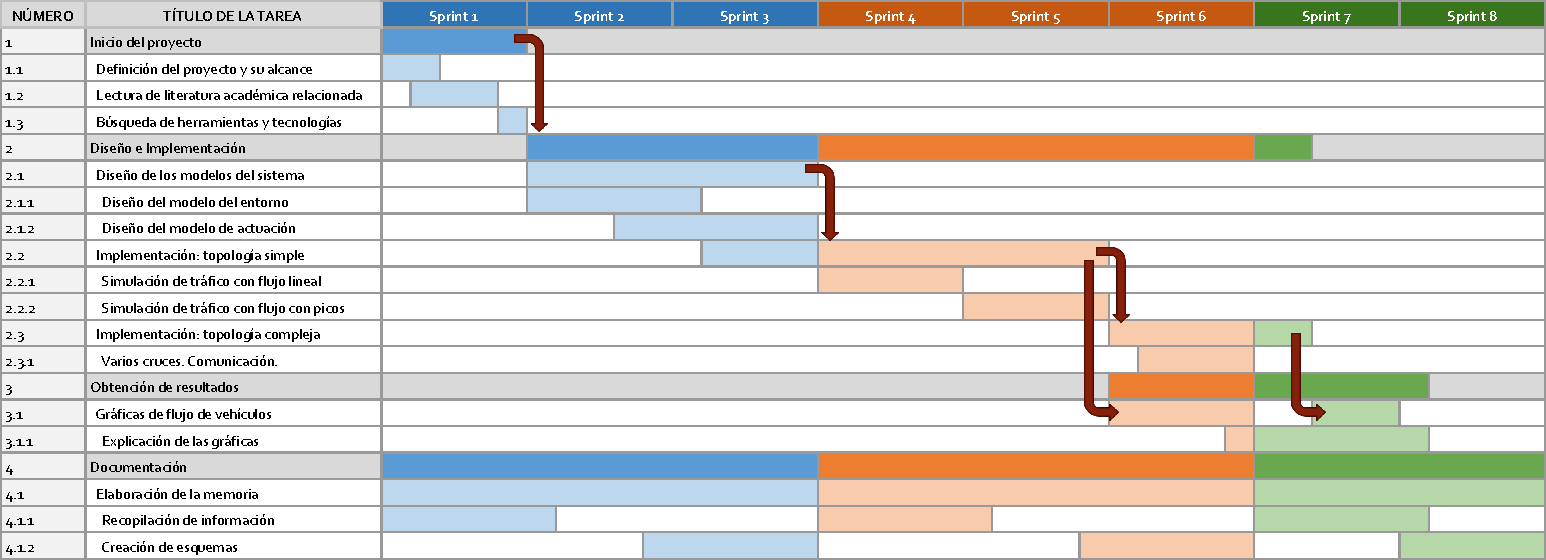
\includegraphics[width=1\linewidth]{text/image/DGantt.pdf}
    \caption{Diagrama de Gantt del proyecto}
    \label{fig:gantt}
\end{figure}

\section{Presupuesto}
La elaboración de un buen presupuesto es una de las partes más importantes en la gestión de proyectos. En multitud de ocasiones, sobre todo si los proyectos son muy grandes, no se tiene un único presupuesto por proyecto, sino que se presupuesta de formas muy variadas, dependiendo, por ejemplo, de la fase en la que se encuentre el proyecto. No es lo mismo que se le quiera proporcionar al cliente un presupuesto inicial, antes de comenzar el proyecto, a que el proyecto se encuentre en una fase avanzada y el cliente solicite nuevas funcionalidades.

Para el proyecto MURAT se ha elaborado un único presupuesto, el cual es suficiente para describir todos los gastos del mismo, los cuales ascienden a un total de 7985 \euro. El presupuesto se ha dividido en tres principales bloques:
\begin{itemize}
    \item \textbf{Personal contratado}: En esta sección se incluyen los gastos conocidos como costes directos, relativos al salario de los empleados. Dentro de esta sección, se pueden diferenciar tres partes principales:
    \begin{itemize}
        \item \textit{Salario bruto}: Es la cantidad total a partir de la cual el trabajador obtiene su sueldo neto previas deducciones por tributación de IRPF y cotización de la Seguridad Social. Se ha estipulado un salario bruto de alrededor de 32.000 \euro \space anuales\footnote{Basado en el sueldo bruto medio de Ingenieros Informáticos en España en el año 2022. Valor obtenido de \href{https://www.glassdoor.es/Sueldos/ingeniero-inform\%C3\%A1tico-sueldo-SRCH_KO0,21.htm}{Glassdoor} a fecha 6 de junio de 2022.}.
        \item \textit{Cuota patronal}: Es la cantidad que la empresa debe pagar por el trabajador. Se compone de los diferentes conceptos: contigencias comunes, 23,60\%; desempleo, 5,50\%; formación profesional, 0,60\%; y FOGASA, 0,20\% \footnote{Basado en el importe mensual que tiene que pagar una compañía en concepto de cuota a la Seguridad Social por tener asalariados contratados. Valores obtenidos de \href{https://www.sdelsol.com/glosario/cuota-patronal/}{Software del Sol} a fecha 6 de junio de 2022.}. Se ha estimado, en total, al 30\% del salario bruto del trabajador.
        \item \textit{Dietas}: Es un extra que en determinadas circunstancias la compañía debe pagar al trabajador. Las dietas son comunes en empresas del sector tecnológico y pueden ser necesarias en cualquier momento. En este caso, no existe ningún gasto relativo a esta parte.
    \end{itemize}
    Este concepto tiene un coste de 6825 \euro \space para el proyecto MURAT.
    \item \textbf{Costes indirectos}: En esta sección se incluyen los gastos generados por el propio ejercicio de la actividad. Es necesario un ordenador portátil, además de un conexión de internet y acceso a la red eléctrica. No  ha sido el caso del proyecto MURAT, aunque en el futuro podría suceder, incurrir en gastos de oficina (o del espacio de trabajo) y de administración, los cuales son prácticamente inherentes a cualquier actividad económica. Este concepto tiene un coste de 1160 \euro \space para el proyecto MURAT.
    \item \textbf{Herramientas y tecnologías}: En esta sección se incluye todo lo relativo a licencias, programas, servicios, etc., necesarios para el proyecto. Esta sección es muy importante en los proyectos de software porque, si bien es cierto que existen muchas herramientas y tecnologías open source gratuitas, existen muchas herramientas y tecnologías propietarias o, incluso, servicios relativos a infraestructura en la nube cuyos costes tienen un impacto considerable en los presupuestos de los proyectos. Este concepto tiene un coste de 0 \euro \space para el proyecto MURAT.
\end{itemize}

\begin{figure}[H]
    \centering
    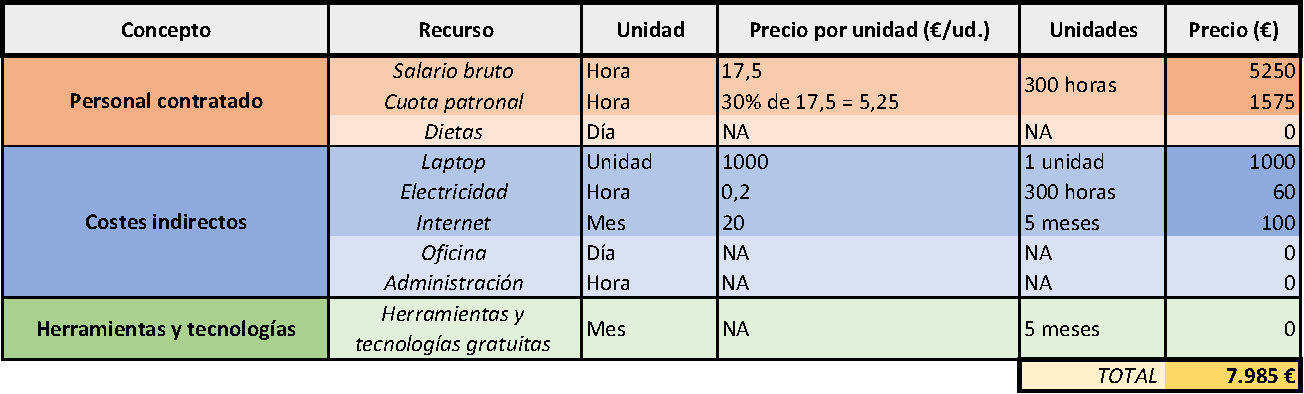
\includegraphics[width=1\linewidth]{text/image/Presupuesto.pdf}
    \caption{Presupuesto del proyecto}
    \label{fig:presupuesto}
\end{figure}